
\secrel{Вводная электронная схема}\label{bcentry}\secdown

\secrel{Где купить комплектующие?}

В Новой Зеландии есть некоторое количество отличных поставщиков компонентов с
разумными ценами, включающих \url{www.surplustronics.co.nz}, и
\url{www.activecomponents.com}. Зарубежные поставщики, которых я использую,
включают \url{www.digikey.co.nz}, \url{www.sparkfun.com}, \url{ebay.com}
и \url{aliexpress.com}.

\bigskip
Для России можно отметить сеть магазинов
``\href{http://voltmaster.ru/}{Больтмастер}''\note{\href{http://voltmaster-samara.ru/}{Самара}}.

\bigskip
Для модулей пока что доступна поставка из Китая по почте:
\href{http://www.aliexpress.com/}{AliExpress}\ с оплатой с виртуальной карты
VISA платежной системы \href{https://qiwi.ru/}{QIWI}. Доставка занимает от 2х
недель до 2х месяцев. Удобно покупать модули в виде микросхем, уже запаянных с
обвязкой на кусок текстолита (\term{breakout board}): Arduino Mini, Maple Mini,
датчики, контроллеры двигателей. Также интересны наборы (магазины) элементов:
пачки резисторов, конденсаторов и т.п. в выводном исполнении, по нескольку
десятков номиналов.

\secrel{Макетная плата: \term{breadboard}}

\begin{youtube}
\url{https://www.youtube.com/watch?v=vQdUSE1auz8}

\url{https://www.youtube.com/watch?v=k9jcHB9tWko}

\url{https://www.youtube.com/watch?v=2wvn8_23phE}

\end{youtube}

\bigskip
\noindent
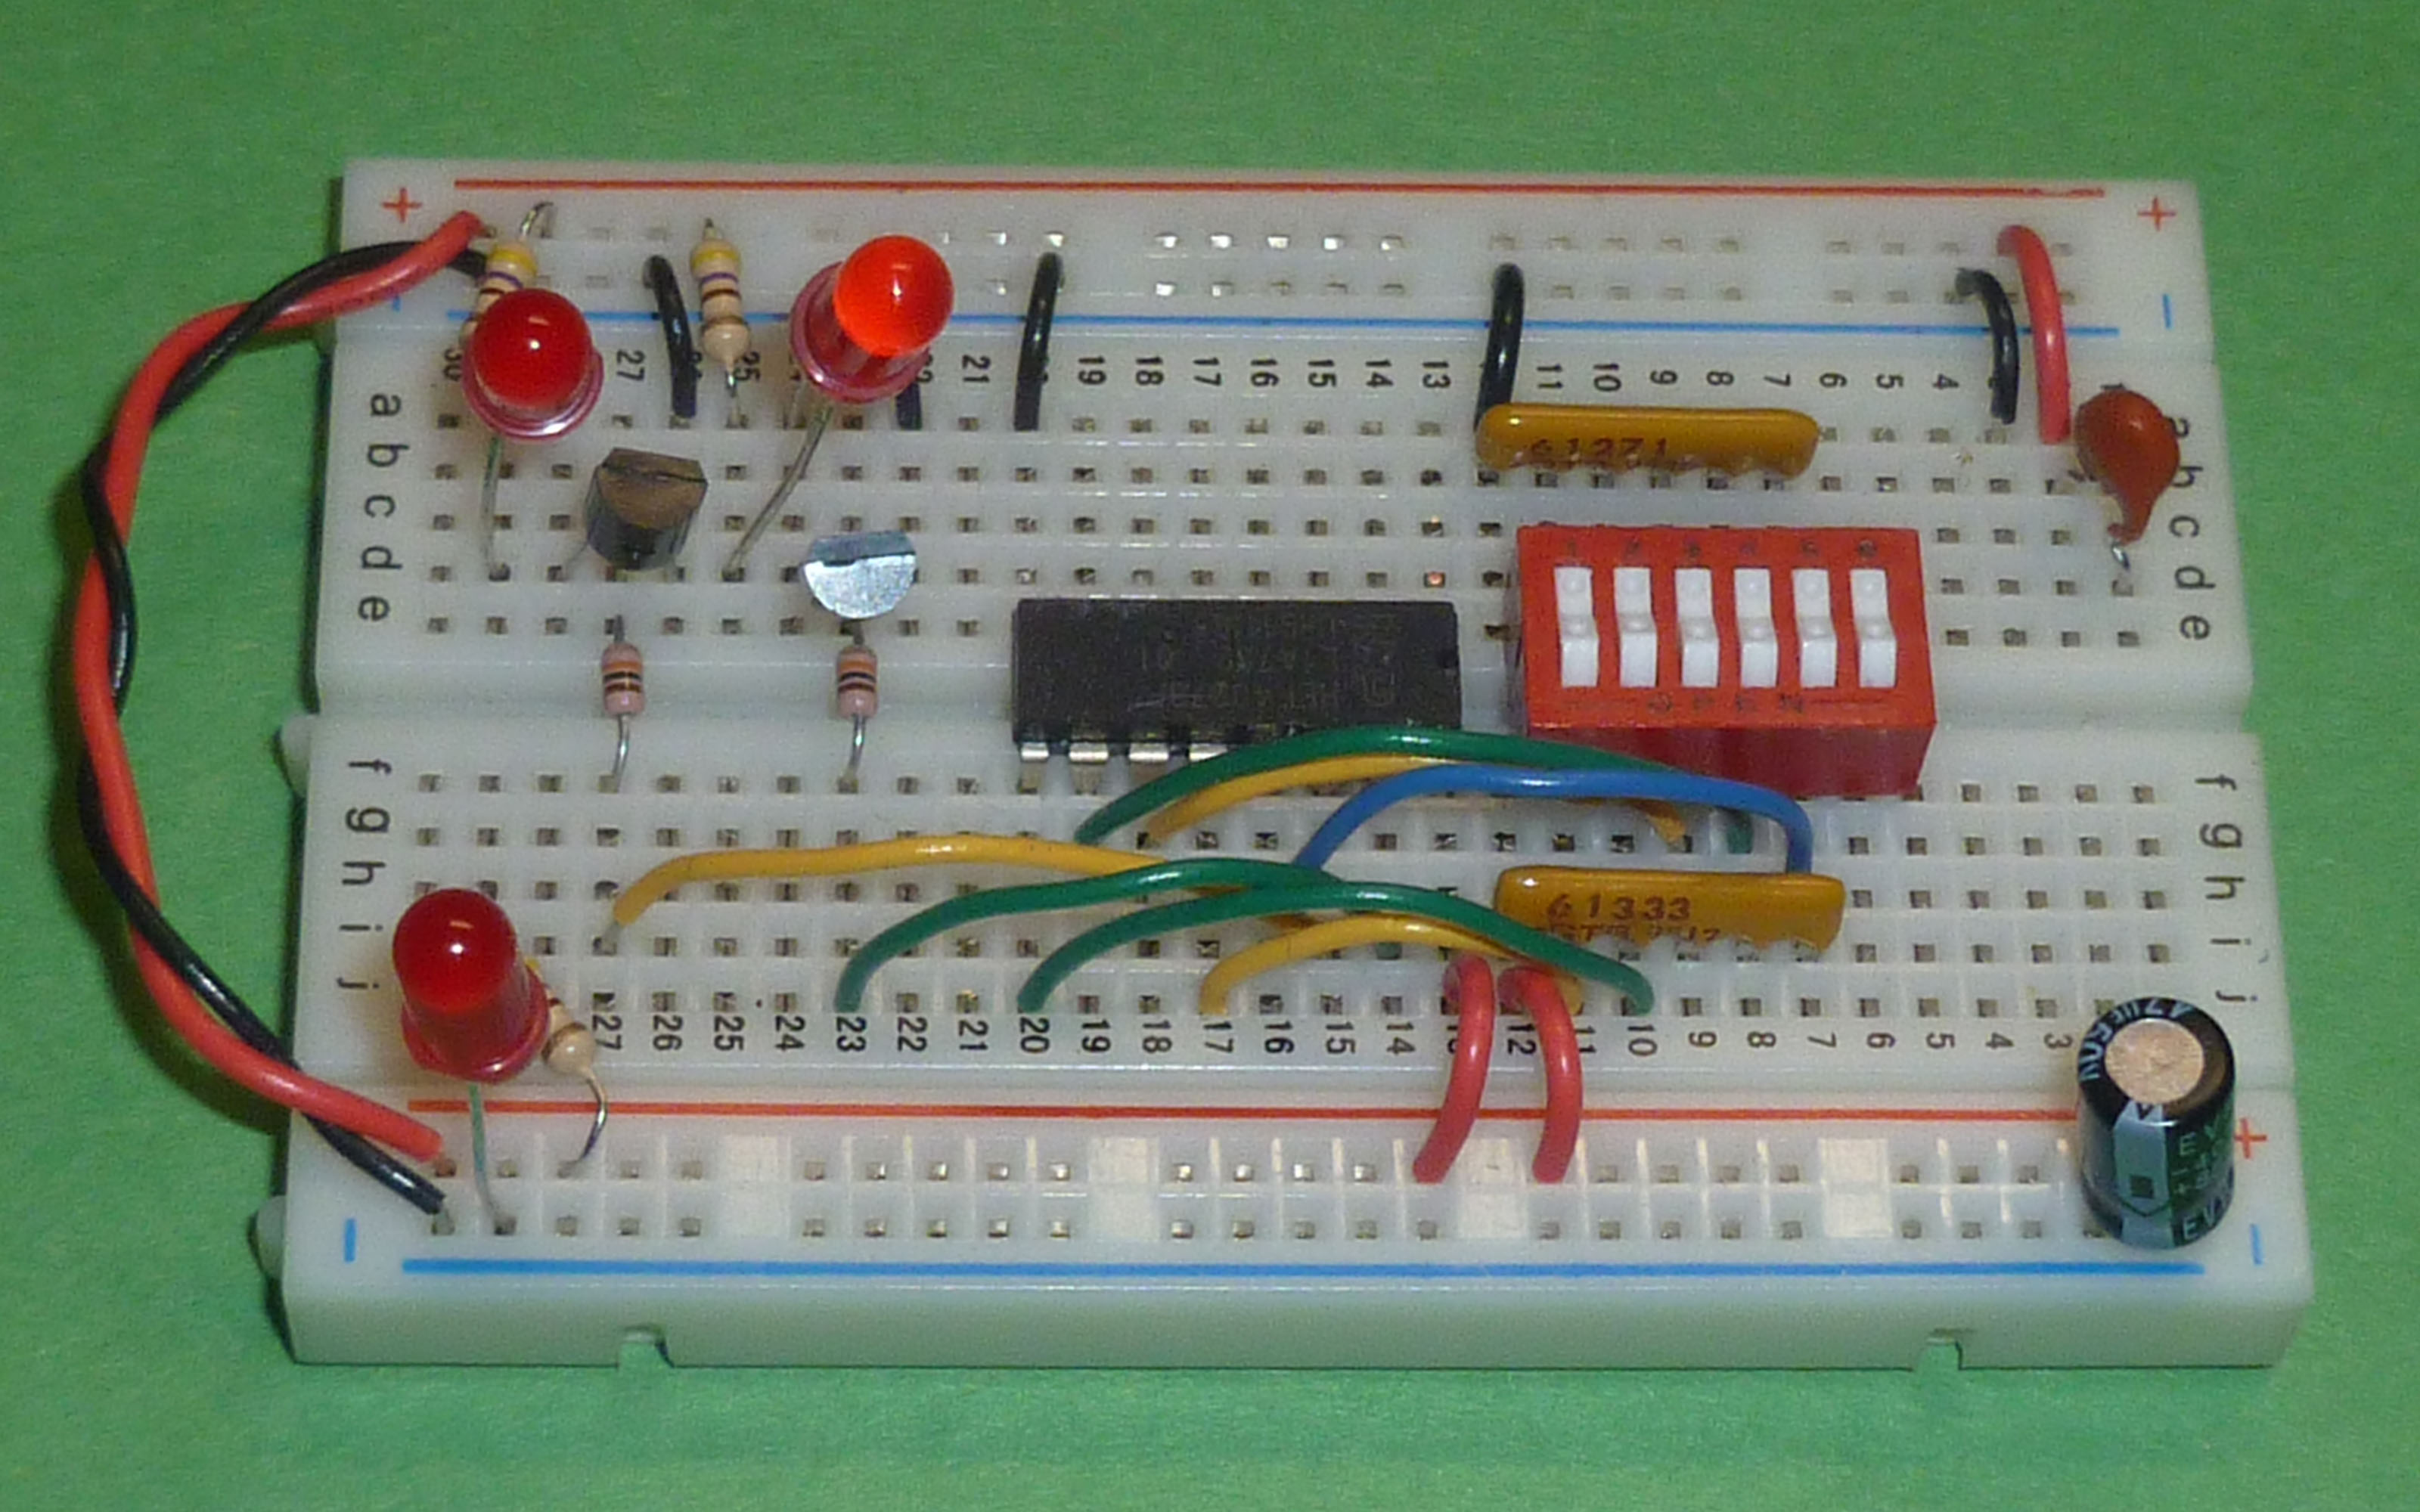
\includegraphics[height=0.3\textheight]{bcollis/breadboard2.jpg}
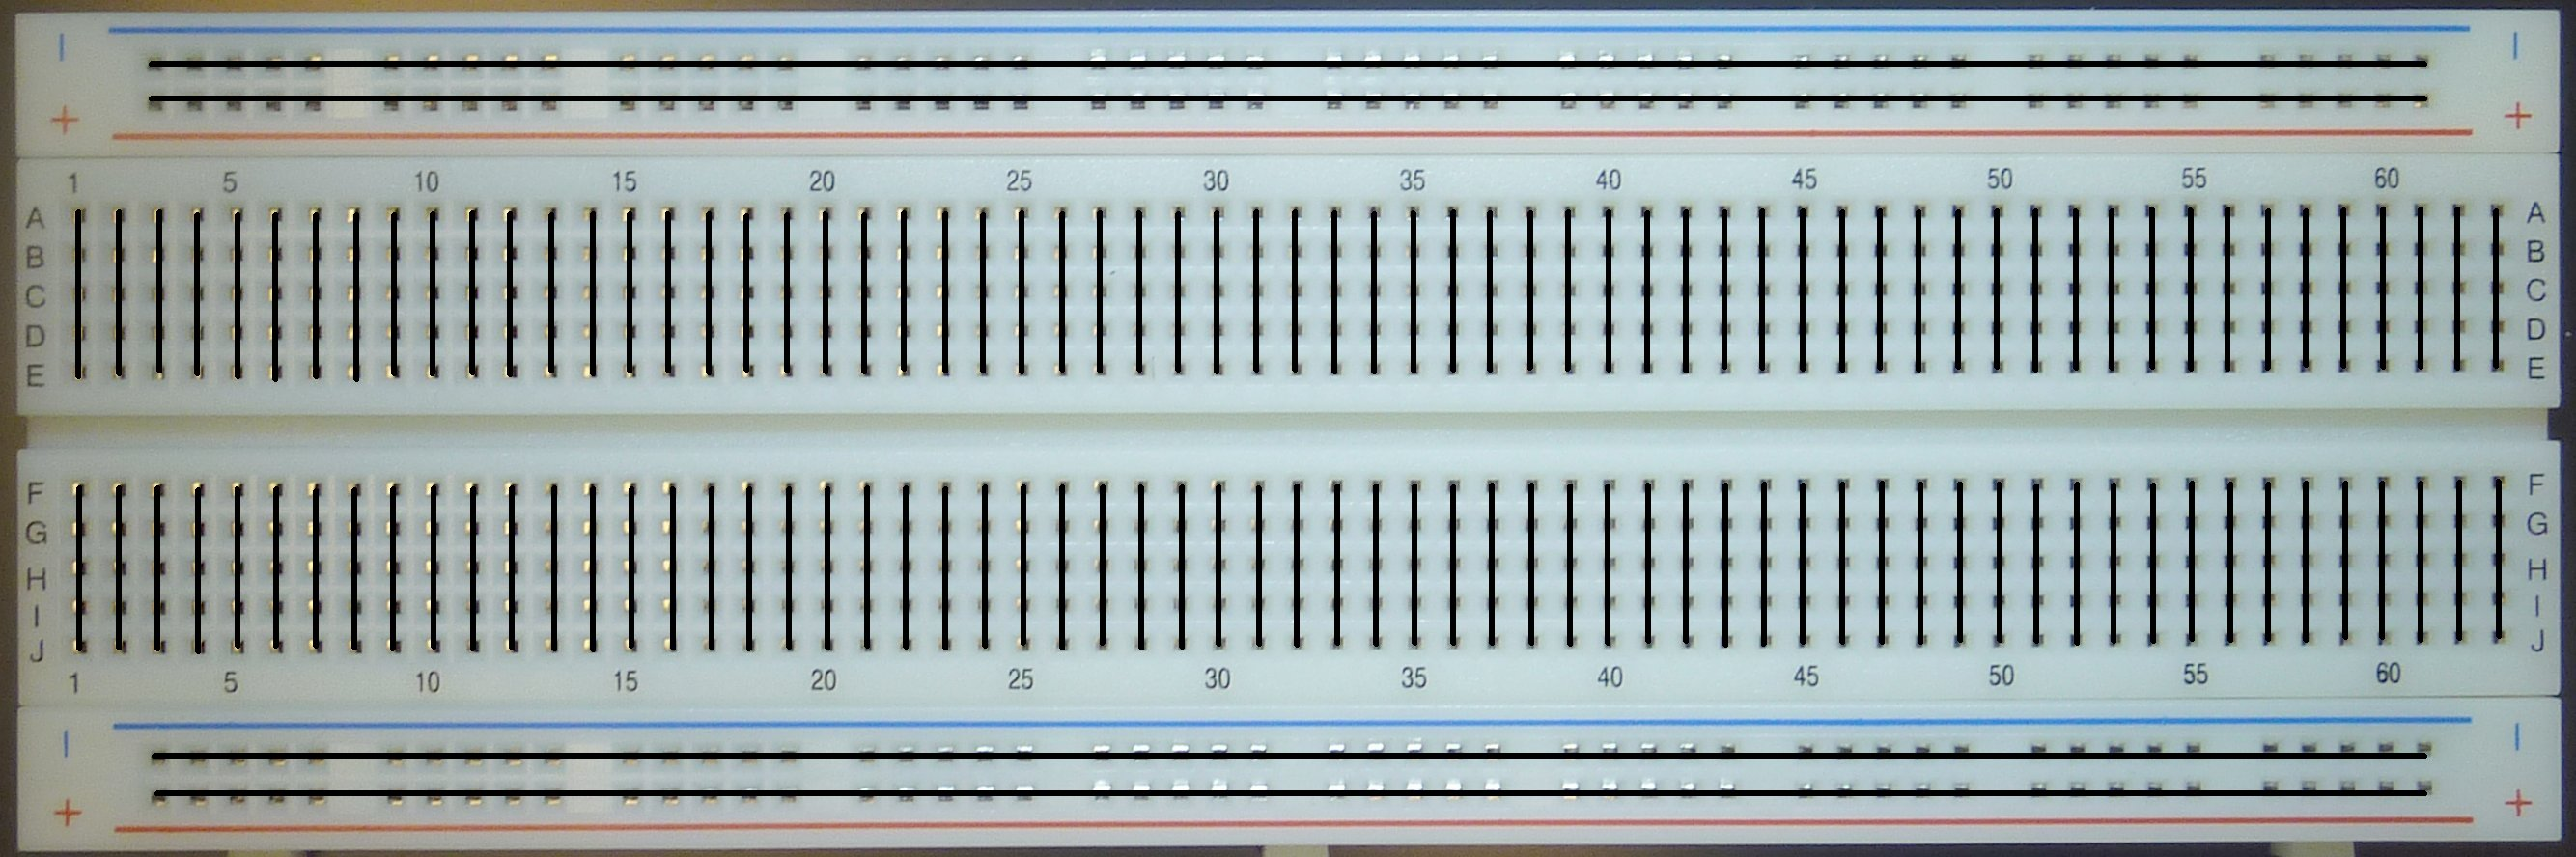
\includegraphics[height=0.3\textheight]{bcollis/BreadboardConnections.jpg}
\bigskip

\termdef{Breadboard}{breadboard} ([б]еспаечная \termdef{[м]акетная
[п]лата}{макетная плата} , \termdef{БМП}{БМП}, ``\termdef{вафля}{вафля}'')\ ---
пластмассовый блок с отверстиями и металлическими полоск\'{о}выми зажимами,
создающими соединения между \termdef{элементами схемы}{элемент}. Отверстия
расположены так, что \termdef{компоненты}{компонент} и отрезки провода могут
быть соединены вместе формируя схему, без использования паяльника. Верхние и
нижние ряды, как правило, используются для \termdef{шин питания}{шина питания},
красный сверху для плюса, и внизу черный/синий для минуса (\termdef{общий
провод}{общий провод}, или \termdef{``земля''}{земля}). На длинных вафлях шины
питания поделены на отдельные сегменты, и требуют соединения короткими
перемычками.

\secrel{Простейшая схема}

Эта схема может быть собрана вот так \ref{ch21lay}, обратите внимание, что
\termdef{светодиод}{светодиод} должен находиться в правильном положении. Если у
вас есть светодиод и \termdef{резистор}{резистор}, соединенные в
\termdef{замкнутый контур}{замкнутый контур}, светодиод должен загореться.

\bigskip
\noindent\begin{tabular}{p{0.45\textwidth} p{0.45\textwidth}}
Принципиальная схема \label{ch21sch}
&
Компоновка \label{ch21lay} \\
&\\
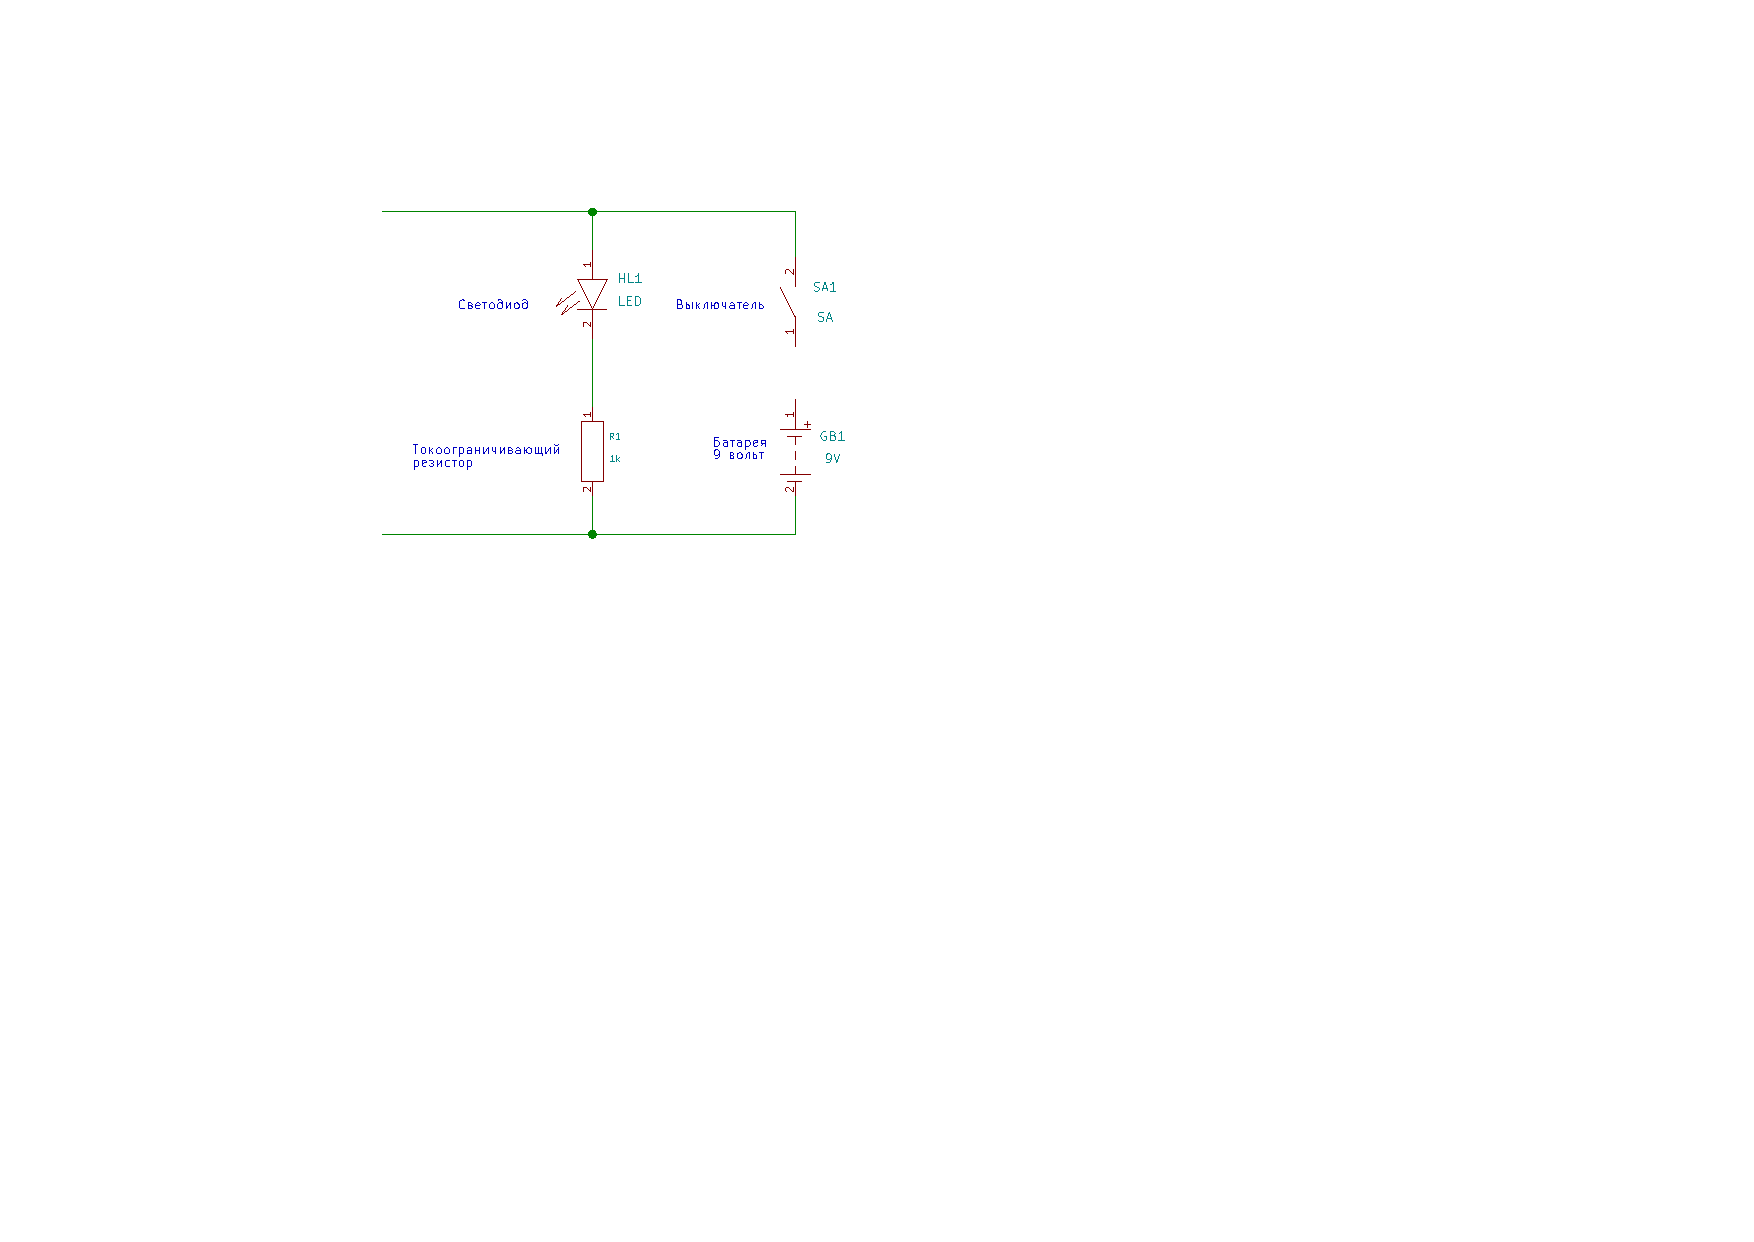
\includegraphics[width=0.45\textwidth]{bcollis/led1/led1.pdf}
&
\\
\end{tabular}

\bigskip
Светодиоду требуется \emph{для включения} около 2\,В\note{[В]ольт}, батарея на
9\,В, так что с напряжением все нормально. \emph{Но если вы подключите светодиод
напрямую к батарее, он сгорит! Для светодиодов главный рабочий параметр\ ---
\termdef{допустимый рабочий ток}{допустимый рабочий ток}, обычно он не превышает
10..20\,mA\note{1\,[м]иллиАмпер = 0.001\,[А]мпер}}. Так что
1\,k\note{1\,[К]илоОм = 1000\,Ом}\ резистор используется для ограничения тока
через светодиод.

\bigskip
Недопустимо подавать на светодиоды напряжение обратной полярности. Светодиоды
имеют невысокое (несколько вольт) обратное пробивное напряжение. В схемах, где
возможно появление обратного напряжения, светодиод должен быть защищён
параллельно включенным обычным диодом в противоположной полярности.

\bigskip
Если вы отключите любой провод в схеме, она перестает работать, схема должна
быть завершенной, чтобы электроны могли течь по проводникам из
\termdef{источника питания}{источник питания}.

\secrel{Ток и напряжение, сечение проводника, плотность тока}\label{bctok}

\begin{youtube}

\url{https://www.youtube.com/watch?v=Dq4fSp6wz-o}

\begin{enumerate}[nosep]
  \item \url{https://www.youtube.com/watch?v=3ZeveDL1\_bg}
  Электрический ток Источники тока
  \item \url{https://www.youtube.com/watch?v=mt86jYUjPFI}
  Ток в металлах Действия электрического тока 
  \item \url{https://www.youtube.com/watch?v=42CEi94hGgA}
  Электрический ток. Сила тока
  \item \url{https://www.youtube.com/watch?v=SNPO5e9wZWU}
  Амперметр Измерение силы тока
  \item \url{https://www.youtube.com/watch?v=Yt91alAwp68}
  Электрическое напряжение
\end{enumerate}

\end{youtube}

В предыдущем разделе были использованы два важных понятия электроники\ ---
\termdef{ток}{ток} и \termdef{напряжение}{напряжение}. Необходимо объяснить эти
понятия, не залезая глубоко в физику. Проще всего объяснить какое-то явление на
примере другого явления, с которым человек регуляроно сталкивается в обыденной
жизни, и ощущает его собственными органами чувств. Для электрических явлений
лучше всего подходит \termdef{гидравлическая модель}{гидравлическая
модель}\note{\href{http://edwpl.ucoz.ru/publ/fundamenty\_ehlektroniki/induktivnye_ehlementy/induktivnosti/5-1-0-18}{пример
применения} гидравлической модели, осторожно, г***осайт}.
В \termdef{ГМ}{ГМ} электрические явления заменяются условными водопроводными:
\termdef{проводник}{проводник}\ --- труба, \termdef{электрический
ток}{электрический ток}\ --- поток воды в этой трубе,
\termdef{резистор}{резистор}\ --- сужение сечения трубы, препятствующее течению
тока, \termdef{диод}{диод}\ --- клапан, открывающися только в одну сторону, и
т.п. В результате маловразумительные абстрактные понятия физики электрических
явлений превращаются в почти ощутимые потоки и давление воды: все мы ежедневно
пользуемся водопроводом, даже в глухих регионах найдется бочка или хотя
бы дырявое ведро.

\bigskip
Таким образом, любому школьнику можно объяснить эти понятия:

\begin{rulebox}
Электрическое \termdef{напряжение}{напряжение}\ --- давление ``электрической
воды'' в проводнике-трубе.\\
Измеряется в \termdef{[В]\'{о}льтах}{Вольт}. 
\end{rulebox}

Как и обычное давление, \emph{напряжение\ --- разностная величина, так как
измеряется между двумя точками} электрической цепи. Для обычного давления за
опорную величину принимают атмосферное давление\note{не ощущаемое человеком, так
как оно уравновешено таким же внутренним давлением крови}. Для электричества
напряжение измеряют тоже между двумя точками, или между точкой и \termdef{общим
проводом}{общий провод}, принимаемым за 0. В физике напряжение определяют также
как \termdef{разность потенциалов}{разность потенциалов} между двумя точками.

\begin{framed}\noindent
Если взять проводник, и разделить его условной плоскостью, перпендикулярной
проводнику, в области пересечения этой плоскости и проводника получается
область\ --- \termdef{сечение проводника}{сечение проводника}.
\end{framed}

Сечение проводника легко увидеть и реально\ --- достаточно взять
толстый одножильный сплошной провод, и аккуратно отпилить (не откусить) его
точно поперек. Поверхность такого отпила и будет сечением.

\begin{rulebox}
Электрический \termdef{ток}{ток}\ --- количество ``электрической
воды'', проходящей через сечение проводника-трубы в единицу времени.
\termdef{Сила тока}{сила тока} измеряется в \termdef{[А]мп\'{е}рах}{Ампер}.
\end{rulebox}

\begin{framed}\noindent
\begin{equation}
j = \frac{I}{S}
\end{equation}
\begin{tabular}{l l l}
где& $j$ & \termdef{плотность тока}{плотность тока}, $\mbox{А}/\mbox{м}^{2}$ \\
&$I$ & сила тока, Ампер \\
&$S$ & \termdef{площадь сечения проводника}{площадь сечения проводника},
$\mbox{м}^{2}$
\end{tabular}
\end{framed}

Чем выше плотность тока, тем больше нагревается проводник (подробнее см
\ref{joul}), поэтому она учитывается при выборе провода, и ширины приводников
печатных плат. В этом случае часто используется численно другая величина\ ---
$\mbox{А}/\mbox{мм}^{2}$.

\secrel{Проводники и изоляторы, сопротивление и проводимость}\label{bcohm}

\begin{youtube}
\begin{enumerate}[nosep]
  \item \url{https://www.youtube.com/watch?v=q4I1hZ5YQ2w}
Электрическое сопротивление проводника.    
  \item \url{https://www.youtube.com/watch?v=SlxOEEaQ4Cg}
Удельное сопротивление 
\end{enumerate}

\url{https://www.youtube.com/watch?v=FCkR-3YE5Ac}

\end{youtube}

Используя гидравлическую модель, точно так же просто можно объяснить понятие
\termdef{проводимости}{проводимость}. Любой материал можно представить как
кусок вещества, имеющий пористую структуру, например как поролон или песок.
Через этот пористый материал течет ``электрическая вода'', т.е. ток. Это течение
вызвано действием напряжения, \term{приложенного} к концам проводника
(источником питания). Напряжение проталкивает электричество через материал,
поэтому чем больше напряжение, тем выше сила проходящего тока. Каждый материал
имееет свою ``пористость'', чем она больше, тем больше \term{проводимость}:

\begin{framed}
\begin{equation}\label{igu}
I = G \ U
\end{equation}
\begin{tabular}{l l l}
где & $I$ & сила тока, А \\
& $G$ & проводимость, См (сименс) \\
& $U$ & напряжение, В \\ 
\end{tabular}
\end{framed}

Чаще вместо проводимости используют обратную величину\ ---
\termdef{сопротивление}{сопротивление}:

\begin{framed}
\begin{equation}
R = \frac{1}{G} = G^{-1}
\end{equation}
\begin{tabular}{l l l}
где & $G$ & проводимость, См (сименс)\\
& $R$ & сопротивление, Ом\\
\end{tabular}
\end{framed}

Соответственно, формула \ref{igu}\ превращается в описанный в любом школьном
учебнике физики \termdef{закон Ома для постоянного тока}{закон Ома!для
постоянного тока}:

\begin{rulebox}
\begin{equation}\label{ohmlaw}
I = \frac{R}{U}
\end{equation}
\end{rulebox}

В зависимости от проводимости или сопротивления материалы делят на несколько
видов:

\bigskip
\begin{tabular}{ l l l }
& $G$, проводимость & $R$, сопротивление \\
\hline
сверхпроводник & $\infty$ & 0 \\ 
\termdef{проводник}{проводник} & большая & низкое \\
\termdef{изолятор}{изолятор}, 
\termdef{диэлектрик}{диэлектрик} & низкая & высокое \\
\end{tabular}
\bigskip

В зависимости от внешних условий: температуры, давления, агрегатного состояния
вещества\note{плазма, газ, жидкость, твердое тело}, примесей\ --- одно и то же
вещество может быть как проводником, так и изолятором.

Типичные проводники: металлы, ионизированный газ (плазма), растворы солей в воде
(электролиты), \emph{влажное} дерево

Типичные диэлектрики: пластики, стекло, керамика, \emph{сухое} дерево, вакуум,
газы в т.ч. воздух.

\bigskip
В электронике очень часто нужно иметь в определенном месте схемы заданное
сопротивление, для этого выпускаются специальные элементы с \emph{точно
калиброванным сопротивлением} между \termdef{выводами}{вывод элемента}:
\termdef{резисторы}{резистор}, иногда применяют устаревшее название \termdef{сопротивление}{сопротивление}
(часто проволочное). Их делают из керамики, на которую наматывают проволоку, или
напыляют тонкую пленку из специальных металлических сплавов с высоким
сопротивлением\note{часто в состав входят никель, хром, вольфрам}.
Иногда используется только кусочек такого сплава без керамики.
Для качественной пайки выводы резисторов делают из хорошо проводящего металла,
хорошо смачиваемого расплавленным припоем.

\secrel{Диэлектрическая и тепловая прочность изоляции}\label{bcisol}

\bigskip
Для диэлектриков существует специальный параметр, характеризующий их способность
работать как изолятор\ --- \termdef{диэлектрическая прочность}{диэлектрическая
прочность}.

\begin{framed}\noindent
Чем выше диэлектрическая прочность, тем большее напряжение способен выдерживать
изолятор без разрушения.
\end{framed}

\begin{framed}\noindent
При повышении температуры диэлектрическая прочность уменьшается 
\end{framed}

Именно поэтому

\begin{alarmbox}
Запрещается использовать любые удлинители в свернутом состоянии, или
использовать электрический провод, свернутый бухтой (катушкой)
\end{alarmbox}

\begin{alarmbox}
Не допускается нагрев любых частей электронной схемы или элементов
конструкции выше 40..50$^{o}C$
\end{alarmbox}

Для любого диалектрика существует некоторое значение напряжения, при котором он
начинает пропускать ток. При прохождении тока материал нагревается (\ref{joul}).
В результате нагрева проходящим током или от соседних соприкасающихся
поверхностей у диэлектрика увеличивается проводимость, что приводит к еще
большему проходящему через него току, и дополнительному нагреву. 

Если тепло не отводится во внешнюю среду (например в середине катушки провода
смотанного удлинителя), температура продолжает повышаться. В некоторый момент
температура достигает значения, при котором слой изоляции размягчается,
утрачивает механическую прочность, и соседние проводники сближаются или
соприкасаются с плохим контактом (происходит \termdef{короткое
замыкание}{короткое замыкание}).

\alarm{В месте плохого контакта или большого тока температура резко повышается}
до значений, когда диалектрик воспламеняется или резко меняет химический состав,
распадаясь \emph{с выделением ядовитых соединений}\note{для типичной изоляции из
ПВХ\ --- сложные токсичные соединения с содержанием хлора} и полностью утрачивая
изолирующие свойства как в электрическом, так и в механическом смысле.

Самый опасный вариант, и типичный случай \termdef{выгорания проводки}{выгорание
проводки}\ --- \termdef{ток короткого замыкания}{ток короткого замыкания}
слишком маленький для срабатывания защитных устройств
(\termdef{предохранитель}{предохранитель}, \termdef{автомат}{автомат},
\termdef{устройство защитного отключения}{устройство защитного
отключения}, \termdef{УЗО}{УЗО}), но достаточный для нагрева изоляции до
температуры химического распада или воспламенения. Аварийного выключения не
происходит, а проводка продолжает гореть до победного конца. 

\secrel{Тепловое действие тока. Мощность}

\begin{youtube}
\begin{enumerate}[nosep]
  \item \url{https://www.youtube.com/watch?v=2LWAIOHRI8s}
  Нагревание проводников электрическим током \termdef{Закон Джоуля Ленца}{закон
  Джоуля Ленца}
  \item \url{https://www.youtube.com/watch?v=Mbt4OTgBRuw}
  \termdef{Мощность}{мощность} электрического тока
\end{enumerate}
\end{youtube}

\secrel{Масштабные множители}\label{bcmux}

\begin{youtube}
\url{https://www.youtube.com/watch?v=i3ABWmCl1EI} Перевод единиц измерения
\end{youtube}

Практически для всех единиц измерения необходимо использование
\termdef{масштабных множителей}{масштабные множители}, когда величины численно
или слишком большие (много цифр до запятой), или слишком маленькие (много цифр
после запятой):

\bigskip
\begin{tabular}{ l l l }
пико & p & $10^{-12}$ \\
nano & n & $10^{-9}$ \\ 
микро & u, $\mu$ & $10^{-6}$ \\ 
милли & m & $10^{-3}$ \\
\hline
кило & k, K & $10^{3}$ \\
мега & M & $10^{6}$ \\
гига & G & $10^{9}$ \\
\end{tabular}
\bigskip

10\,mA = $10 \times 10^{-3}$\ A = $10 \times 0.001$ A = 0.010 A

5\,КОм = $5 \times 10^{3}$ Ом = $5 \times 1000$ Ом = 5000 Ом

\secrel{Использование мультиметра}\label{bcmmetr}

\begin{youtube}
\url{https://www.youtube.com/watch?v=BEgvm4o-u2Q}

\url{https://www.youtube.com/watch?v=UMwYLwsPgCY}

\begin{enumerate}[nosep]
  \item \url{https://www.youtube.com/watch?v=GBuGSj1uPGk}
  \item \url{https://www.youtube.com/watch?v=VJ3RBS42IVY}
\end{enumerate}

\url{https://www.youtube.com/watch?v=q3R4s6WE1cI}
\end{youtube}

Возьмите мультиметр (\ref{mmetr}) и измерьте напряжение на резисторе, близко ли
оно к 7\,В ? Также измерьте ток через диод, не превышает ли он допустимый ?

\begin{framed}
\emph{Напряжение} измеряется \term{в [В]\'{о}льтах} подключением
\term{измерительного прибора} (мультиметра) \emph{параллельно}\ элементу, при этом нужно
\begin{itemize}
\item
\term{режим измерения} включить на
\term{режим измерения постоянного напряжение} $V-$/DCV (или переменного,
обозначается как $V\sim$/ACV) а
  \item \term{диапазон
измерения} \emph{выставить на максимальное значение напряжения}
\item
Последовательно уменьшая диапазон измерения, найдите диапазон, в котором
мультиметр показывает наибольшее количество знаков после запятой.
\end{itemize}
\end{framed}

Если диапазон
слишком большой, прибор покажет значение в районе 0, а если слишком низкий\ ---
выведет [1]. Обычно работают в диапазоне, соответствующем максимальому
напряжению питания (в нашем случае 20\,V\note{[V]olt = [В]ольт}), иногда для
слабых напряжений переключаясь на одну..две ступени ниже. Но\ ---
\emph{возможны случаи\note{в \emph{любых схемах} содержащих
\term{индуктивности}: катушки пр\'{о}вода, трансформаторы, электродвигатели,
динамики и т.п.} когда напряжение в части схемы на порядки (в десятки..тысячи
раз) превосходит напряжение питания}.

\begin{framed}
\emph{Ток} измеряется \term{в [А]мп\'{е}рах} подключением \term{измерительного
прибора} (мультиметра) \emph{последовательно}\ с элементом \term{в разрыв цепи}, при этом
нужно
\begin{itemize}
\item
\term{режим измерения} включить на
\term{режим измерения постоянного тока} $A-$/DCA (или переменного, обозначается
как $A\sim$/ACA) а
  \item \term{диапазон
измерения} \emph{выставить на максимальное значение тока}
\item
Последовательно уменьшая диапазон измерения, найдите диапазон, в котором
мультиметр показывает наибольшее количество знаков после запятой.
\end{itemize}
\end{framed}

Обратите внимание, что напряжение измеряется \term{вольтметром} на полностью
собранной схеме, а для измерения тока нужно изменять схему, включая в нее
\term{амперметр}. Если измерения тока нужно проводить на готовом устройстве,
иногда ставят 2хконтактный \term{джампер} (как на материнских платах
компьютеров): при измерении амперметр подключают к его контактам, а потом
джампер замыкают специальной съемной проводящей перемычкой. Этом прием вы можете
использовать в своих устройствах для регулярного измерения \term{тока
потребления}, и расчета \term{потребляемой мощности}:

\begin{equation}
W_{\mbox{потребляемая}}\mbox{[Ватт]} =
U_{\mbox{питания}}\mbox{[Вольт]}
\times
I_{\mbox{устройства/элемента}}\mbox{[Ампер]}
\end{equation}

\begin{framed}
Переключив мультиметр в \term{режим прозвонки (т\'{е}стера)}, можно проверить
\begin{itemize}
\item наличие
электрического соединения между двумя точками \emph{обязательно отключенной от
источника питания} схемы,
\item исправность диода или светодиода,
\item исправность конденсатора большой \term{емкости} и
\item любые другие случаи когда нужно определить что две точки электрически
соединены между собой, постоянно или временно.
\end{itemize}
\end{framed}

Если между \term{щщуп}ами мультиметра в режиме прозвонки\note{= тестера}\
\term{сопротивление} протекающему току не превышает 1\,КилоОм\note{см.
паспорт на прибор}, раздается звуковой сигнал.

Если щщупы подключить к исправному \emph{разряженному} конденсатору большой
емкости (``электролиту''), раздастся короткий целчок или даже ``пик''.

Тестером также можно определить тип и \term{цокол\'{е}вку\note{``раскопытку''}}
транзистора; как это сделать описано в \ref{vt}.

\emph{Диоды} проверяются двумя подключениями \emph{в разной полярности}\ --- при
\emph{красном щщупе} на \term{аноде (+)} диода (в \term{прямой полярности
включения}) диод проводит ток, а в \term{обратной полярности} нет (красный щщуп
на \term{катоде (-)}).

Проверьте \emph{светодиод}: отключите его из схемы, и проверьте как диод.
Если светодиод исправен, в \emph{прямой полярности} светодиод будет \emph{очень
слабо светиться}.

\secrel{Определение сопротивления резистора по цветовому коду}

Когда берете резистор, проверьте его \termdef{номинал}{номинал} (значение). В
наших схемах каждый резистор имеет свою цель, и значение выбирается в
зависимости от того, хотим ли мы б\'{о}льший или меньший ток в этой части цепи.
Чем выше \term{номинал} резистора, тем меньше ток. Чем ниже номинал резистора,
тем выше ток. Для \termdef{выводн\'{ы}х}{выводн\'{о}й корпус} резисторов,
которые мы будем использовать на макетках, маркировка наносится на корпус в
виде набора цветных полосок:

\bigskip
Цветовая маркировка на 5 цветных полосок:
\begin{tabular}{|l|l|l|l|l|}
\hline
 цифра & цифра & цифра & множитель & точность \\
\hline
\end{tabular}

\bigskip Цифра:
\begin{tabular}{l l l l l l l l l l}
0&1&2&3&4&5&6&7&8&9\\
\textcolor{Black}{$\blacksquare$} &
\textcolor{Brown}{$\blacksquare$} &
\textcolor{Red}{$\blacksquare$} &
\textcolor{Orange}{$\blacksquare$} &
\textcolor{Yellow}{$\blacksquare$} &
\textcolor{Green}{$\blacksquare$} &
\textcolor{Blue}{$\blacksquare$} &
\textcolor{Magenta}{$\blacksquare$} &
\textcolor{Grey}{$\blacksquare$} &
$\square$ \\
\end{tabular}

\bigskip Множитель:
\begin{tabular}{l l l l l l l l l l}
\textcolor{Black}{$\blacksquare$} & $10^{0}=1$ &
\textcolor{Brown}{$\blacksquare$} & $10^{1}=10$ &
\textcolor{Red}{$\blacksquare$} & $10^{2}=100$ &
\textcolor{Orange}{$\blacksquare$} & $10^{3}=1000$ \\
\textcolor{Yellow}{$\blacksquare$} & $10^{4}=10000$ &
\textcolor{Green}{$\blacksquare$} & $10^{5}=100000$ &
\textcolor{Blue}{$\blacksquare$} & $10^{6}=1000000$ \\
\textcolor{Gold}{$\blacksquare$} & $10^{-1}=0.1$ &
\textcolor{Silver}{$\blacksquare$} & $10^{-2}=0.01$ \\
\end{tabular}

\bigskip Точность:
\begin{tabular}{l l l l l l l l l l l}
\textcolor{Brown}{$\blacksquare$} & $\pm 1\%$ &
\textcolor{Red}{$\blacksquare$} & $\pm 2\%$ &
\textcolor{Gold}{$\blacksquare$} & $\pm 5\%$ &
\textcolor{Silver}{$\blacksquare$} & $\pm 10\%$ \\
\end{tabular}

\bigskip
\begin{tabular}{l l l l l l l l l l l l l}
-[&
\textcolor{Brown}{$\blacksquare$}&
\textcolor{Black}{$\blacksquare$}&
\textcolor{Black}{$\blacksquare$}&
\textcolor{Yellow}{$\blacksquare$}&
\textcolor{Brown}{$\blacksquare$}&
]- 
& $100\times 10^{4}\pm 1\%$ & 1M & 1 миллион Ом & 1M $\Omega$ & 1 000 000 Ом \\
&1&0&0&4&1\\
-[&
\textcolor{Brown}{$\blacksquare$}&
\textcolor{Black}{$\blacksquare$}&
\textcolor{Black}{$\blacksquare$}&
\textcolor{Red}{$\blacksquare$}&
\textcolor{Red}{$\blacksquare$}&
]- 
& $100\times 10^{2}\pm 2\%$ & 10k & 10 тысяч ом & 10,000 Ом & 10k $\Omega$ \\
&1&0&0&2&2\\
-[&
\textcolor{Brown}{$\blacksquare$}&
\textcolor{Black}{$\blacksquare$}&
\textcolor{Black}{$\blacksquare$}&
\textcolor{Brown}{$\blacksquare$}&
\textcolor{Gold}{$\blacksquare$}&
]- 
& $100\times 10^{1}\pm 5\%$ & 1k & 1 тысяча ом & 1000 Ом & 1k $\Omega$ \\
&1&0&0&1&5\\
-[&
\textcolor{Orange}{$\blacksquare$}&
$\square$&
$\blacksquare$&
\textcolor{Black}{$\blacksquare$}&
\textcolor{Brown}{$\blacksquare$}&
]- 
& $390\times 10^{0}\pm 1\%$ & 390R & 390 Ом & 390$\Omega$ \\
&3&9&0&0&1\\
-[&
\textcolor{Brown}{$\blacksquare$}&
\textcolor{Black}{$\blacksquare$}&
\textcolor{Black}{$\blacksquare$}&
\textcolor{Black}{$\blacksquare$}&
\textcolor{Brown}{$\blacksquare$}&
]- 
& $100\times 10^{0}\pm 1\%$ & 100R & 1000 Ом & 100$\Omega$ \\
&1&0&0&0&1\\
-[&
\textcolor{Yellow}{$\blacksquare$}&
\textcolor{Magenta}{$\blacksquare$}&
\textcolor{Black}{$\blacksquare$}&
\textcolor{Gold}{$\blacksquare$}&
\textcolor{Brown}{$\blacksquare$}&
]- 
& $470\times 10^{-1}\pm 1\%$ & 47R & 47 Ом & 47$\Omega$ \\
&4&7&0&-1&1\\
\end{tabular}

\secrel{Светодиоды}

\noindent
\begin{tabular}{p{0.7\textwidth}p{0.3\textwidth}}
\noindent\parbox[b]{0.65\textwidth}{В настоящее время светоизлучающие диоды
используются в индикаторах и дисплеях на различном оборудовании, однако они все
больше и больше используются в качестве замены для \termdef{галогенных
ламп}{лампа!галогенная} и \termdef{ламп
накаливания}{лампа!накаливания}\note{использующие светящиеся проводники внутри
стеклянных колб} во многих других приложениях. Они включают в себя ходовые огни
на транспорте, светофоры,  большие уличные TV-экраны.}&
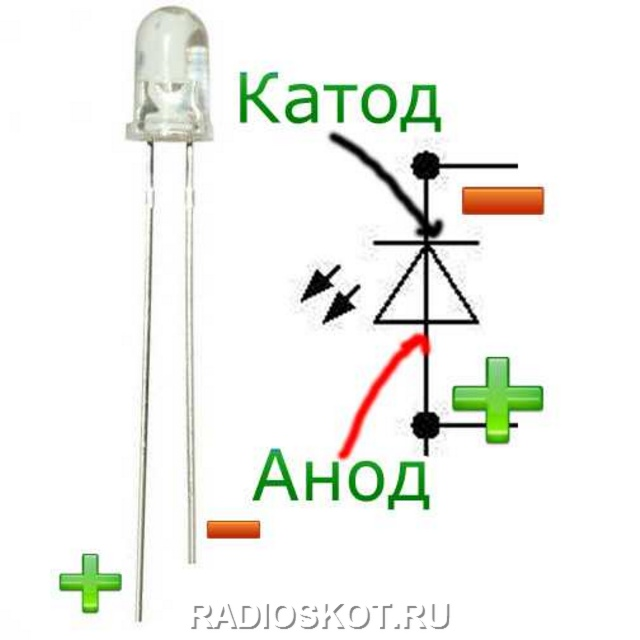
\includegraphics[width=0.25\textwidth]{bcollis/led.jpeg}
\\
\end{tabular}

\noindent
\begin{tabular}{p{0.3\textwidth} p{0.7\textwidth}}
\noindent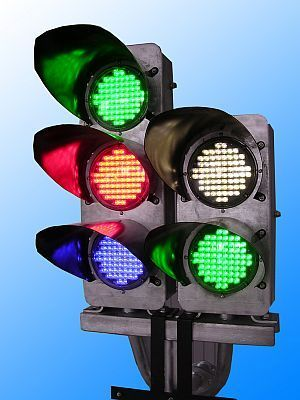
\includegraphics[width=0.3\textwidth]{bcollis/ledtraffic.jpeg}&
\noindent\parbox[b]{0.65\textwidth}{По сравнению с \term{лампами накаливания},
светодиоды почти не дают тепла, и поэтому очень эффективны. Они также имеют
гораздо б\'{о}льшее время жизни, например 10 лет, по сравнению с 10 месяцами для
ламп накаливания. Таким образом, в некоторых ситуациях например сигналов
светофора, если там установлены светодиоды, они дают значительную экономию как
по потребляемой мощности, так и по стоимости технического обслуживания. Хотя
есть небольшая проблема со светодиодными светофорами\ --- они не плавят снег,
который на них налипает!}\\
\end{tabular}

\secrel{Некоторые характеристики светодиодов}

\paragraph{\termdef{Интенсивность}{интенсивность}}: измеряется в мКд
(милликанделлах)

\paragraph{\termdef{Угол обзора}{угол обзора}}: угол от оси, до линии, где
интенсивность падает до 50\%

\paragraph{\termdef{Прямое напряжение}{прямое напряжение!светодиода}}:
напряжение необходимое для получения полной яркости светодиода

\paragraph{\termdef{Прямой ток}{прямой ток!светодиода}}: рабочий ток, дающий
максимальную яркость

\paragraph{\termdef{Пиковая длина волны}{пиковая длина волны}}: самая яркая
спектральная линия излучаемого света

\secrel{Задание на исследование светодиода}

Пользуясь сайтом одного из поставщиков, найдите информацию и
характеристики/атрибуты для двух светодиодов: обычный красный 5 мм и 5 мм
высокой интенсивности.


\bigskip
\begin{tabular}{|l|p{0.3\textwidth}|p{0.3\textwidth}|}

Cветодиод
&
Красный 5\,мм
&
Высокая интенсивность 5\,мм
\\
\hline

Поставщик&&\\

Номер детали&&\\

Стоимость (\$)&&\\

Яркость (мКд)&&\\

Прямое напряжение ($U_{F}$)&&\\

Длина волны (нм)&&\\

Прямой ток ($I_{F}$)&&\\

\end{tabular}

\clearpage\secrel{Добавление выключателя в схему}

Выключатель\ --- способ для ручного управления схемой пользователем

\bigskip\noindent
\begin{tabular}{p{0.45\textwidth} p{0.45\textwidth}}
Принципиальная схема
&
Компоновка
\\
\noindent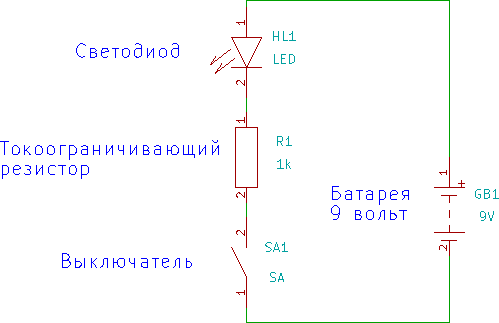
\includegraphics[width=0.45\textwidth]{bcollis/led2/led2.pdf}
&
\\
\end{tabular}

\secrel{2.7 Задание на установку выключателя 18}

2.7 Switch assignment

Find a small switch and carefully disassemble it (take it apart) draw how it
works and explain its operation. Make sure you explain the purpose of the
spring(s).

Here are simplified drawings of a small slide switch when it is in both
positions. When the switch is on electricity can flow, when it is open the
circuit is broken.


\secrel{Важные понятия схемотехники}

Кратко повторим:
\bigskip

Схема состоит из нескольких компонентов и источника питания, соединенных
проводами.

\emph{Поток электронов} (часто называют \termdef{носители заряда}{носители
заряда}) течет в цепи; однако если нет \emph{полной (замкнутой) цепи}, электроны
не могут течь.

\emph{Напряжение} (U) является мерой энергии в цепи, оно используется в качестве
меры энергии, подаваемой от батареи или энергии (напряжения) через часть схемы.

\emph{Ток (I) представляет собой поток электронов} от батареи по контуру и
обратно к батарее. Ток измеряется в амперах (обычно мы будем использовать
миллиампер или мА). Обратите внимание, что \emph{электрический ток это не ток
электронов или ток зарядов}. Так же, как течение реки не эквивалентно потоку
воды.

\emph{Сопротивление} работает \emph{на уменьшение тока}, резисторы в схеме
оказывают сопротивление току.

\emph{Проводники}, такие как провода, соединяющие компоненты вместе, не имеют
(теоретически) никакого сопротивления току.

\bigskip
Действительно важное понятие, для ясного понимания:

Напряжение прикладывается параллельно компонентам, а ток течет через компоненты.

\secrel{Изменение величины сопротивления}

Каков эффект изменения значения сопротивления в нашей цепи?

Резистор контролирует ток, чем выше значение резистора, тем меньше ток.
Как будет выглядеть резистор на 10K?

\bigskip\begin{tabular}{l l l}
390R & больший ток & яркое свечение светодиода \\
1k & слабый ток & тусклое свечение \\
1M & нет тока & нет свечения \\
\end{tabular}


\secrel{2.10 Добавление транзистора в схему 20}

2N7000

\bigskip
\termdef{Транзистор}{транзистор}\ --- электронный элемент, выполняющий функцию
\termdef{усиления}{усиление}: \emph{управление сильным сигналом под контролем
слабого сигнала}.

\bigskip
Частный случай транзистора\ --- \termdef{Полевой транзистор}{полевой транзистор} 
(\termdef{FET}{FET}, [F]ield [E]ffect [T]ransistor). Управление выполняется
слабым входным \emph{напряжением}, которое управляет выходным током, изменяя
проводимость (сопротивление) части транзистора в выходной цепи. 

Главная особенность полевого транзистора\ --- во входной цепи, по которой
подается управляющее напряжение, течет почти нулевой \termdef{входной
ток}{входной ток}, т.е. \emph{полевой транзистор имеет бесконечное
\termdef{входное сопротивление}{входное сопротивление}}. Эта особенность важна
при подключении источников слабого сигнала (датчиков), генерирующих слабое
сигнальное напряжение, но не способных выдать сколь нибудь заметный ток\ ---
электро-динамический микрофон, индуктивный звукосниматель электрогитары и т.п.
Сигнал от таких датчиков усиливается \termdef{предварительным
усилителем}{предварительный усилитель} на полевом транзисторе, а затем усиленный
сигнал подается в остальную часть схемы для дальнейшей обработки.

\secrel{Понимание схем}

Электроника\ --- все что относится к управлению в физическом мире. Физические
объекты имеют свойства, такие как температура, сила, движение, и
звуковые/радио/световые колебания, связанные с ними.

\bigskip
Электронные устройства имеют \termdef{входные цепи}{входная цепь}, чтобы
преобразовать физический мир (свет, звук и т.д.) в различные уровни напряжения. 

Они включают в себя \term{преобразующие схемы}, которые преобразуют,
манипулируют и изменяют информацию (информация закодирована в виде различных
напряжений).

Они имеют \termdef{выходные цепи}{выходная цепь} для преобразования различных
уровней сигнала обратно в физический мир, где мы можем почувствовать результат
процесса (свет, звук и т.д.)

\bigskip
Рассмотрим пример, например телевизор: радиосигнал из физического мира на входе
преобразуется электронной схемой в уровень напряжения, и преобразуется в свет,
который мы видим, и звук, который можно слышать.

\secrel{Входная цепь\ --- фоторезистор (LDR)}

\begin{tabular}{p{0.62\textwidth} l}
\parbox[b]{0.62\textwidth}{
LDR\note{Light Dependent Resistor} или фоторезистор\ --- типичный компонент,
используемый в цепях измерения уровня освещенности. LDR изменяет сопротивление
пропорционально интенсивности света, падающего на него. Фоторезисторы
изготавливаются из полупроводников, таких как селен, оксид таллия и сульфид
кадмия. Когда фотоны света сталкиваются с атомами в материале LDR, проводимость
увеличивается, и электроны могут течь через цепь. Это означает, что по мере
увеличения уровня освещенности, сопротивление уменьшается.

\bigskip
Фоторезисторы можно использовать только с маленьким протекающим через него током
порядка 5\,мА, если превышается допустимый ток, LDR перегревается и сгорает.
Обычно они используются в схеме делителя напряжения последовательно с обычным
резистором.
}
&
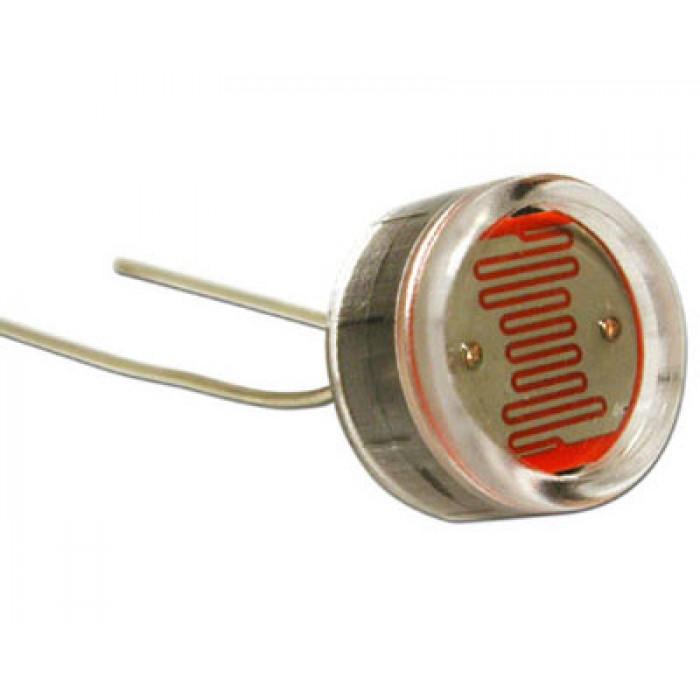
\includegraphics[width=0.3\textwidth]{bcollis/LDR.jpg}
\end{tabular}
\bigskip

Найдите фоторезистор и измерьте его сопротивление:

сопротивление LDR при полном дневном свете \verb|__________|

сопротивление LDR в темноте \verb|__________|

\bigskip
\begin{tabular}{l l}
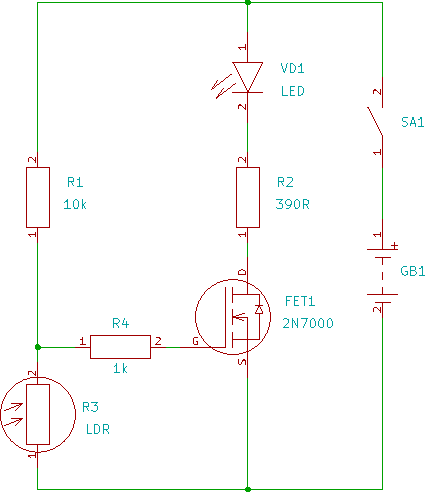
\includegraphics[height=0.65\textheight]{bcollis/ldr/ldr.pdf}
&\\
\end{tabular}
\bigskip

Компоненты на схеме: резистор R1 от 10K (10 000)\,Ом до 1M (1 000 000)\,Ом,
R3 фоторезистор, GB1 батарея. R1, R3\ --- схема делителя напряжения (питания),
резистор R2 ограничивает ток через светодиод VD1 и цепь исток/сток полевого
транзистора.

В темноте LDR имеет высокое сопротивление, и напряжение на выходе высокое.

На свету LDR имеет низкое сопротивление, и напряжение падает.


\secrel{Рабочая схема датчика темноты}

Экспериментируя с резистором последовательно с LDR, можно регулировать
чувствительность схемы на различных уровнях освещенности.

\secrel{Защитные цепи\ --- использование диода}

Диоды очень часто используемые компоненты, они бывают всех форм и размеров.

\begin{framed}\noindent
Диод\ --- электронный прибор, пропускающий ток только в одном направлении
\end{framed}

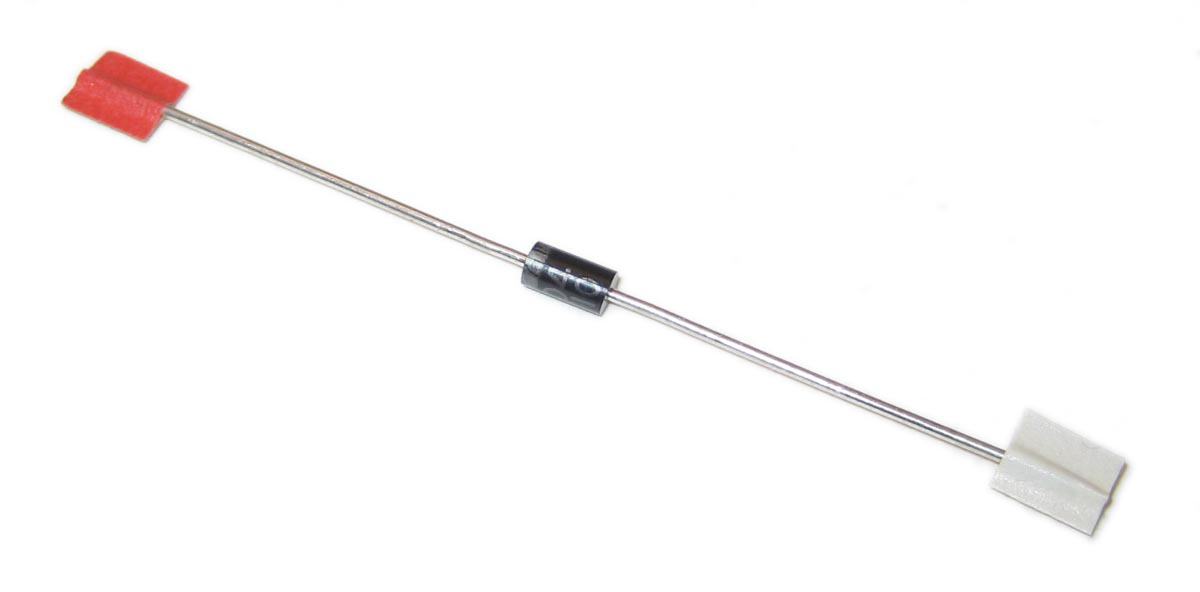
\includegraphics[height=0.3\textheight]{bcollis/vd/1N4004.jpg}
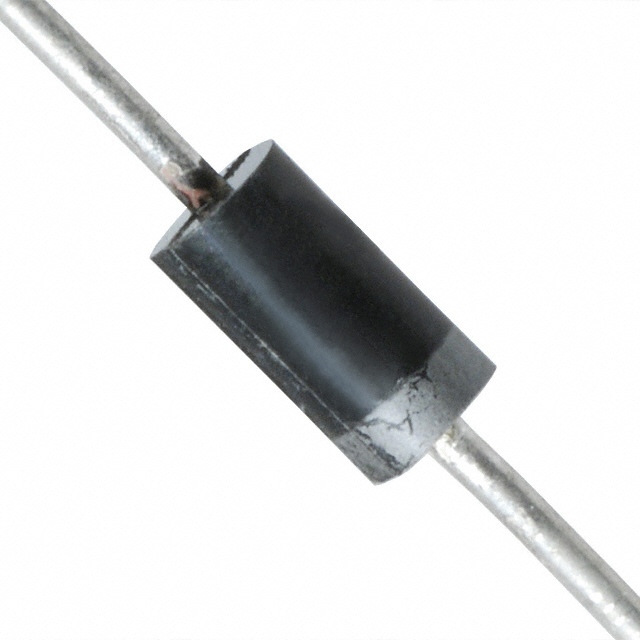
\includegraphics[height=0.3\textheight]{bcollis/vd/1N4007.jpg}
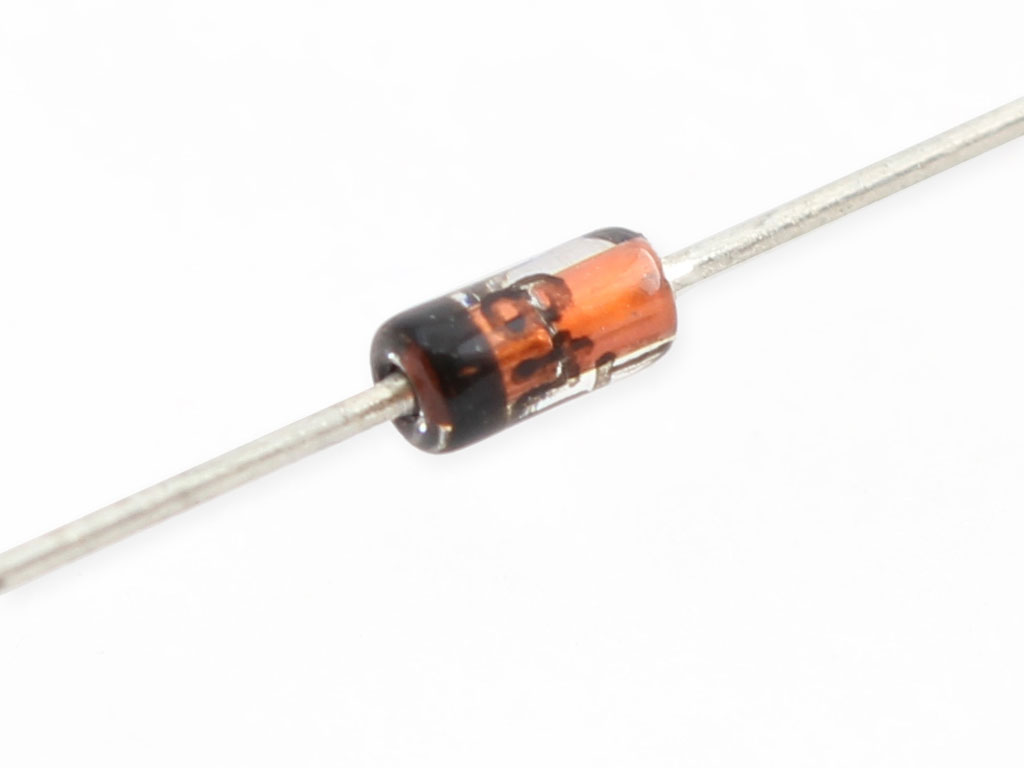
\includegraphics[height=0.3\textheight]{bcollis/vd/1N4148.jpg}

\noindent
\begin{tabular}{p{0.45\textwidth} p{0.45\textwidth}}
\noindent
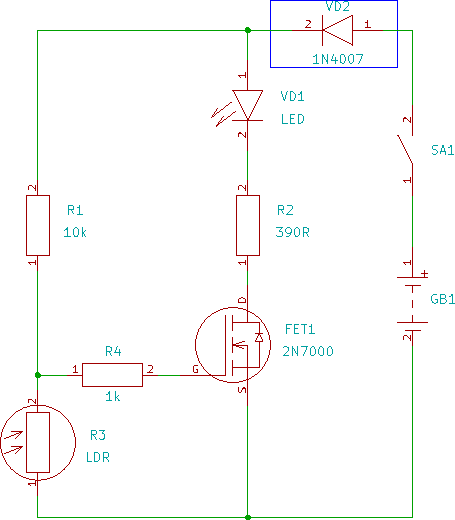
\includegraphics[width=0.45\textwidth]{bcollis/vd/vd.pdf}
&
\parbox[b]{0.5\textwidth}{
Основная характеристика диода\ --- то что ток течет только в одном направлении,
так что вы не можете его пустить в схеме в обратном направлении, и можете быть
уверены, что это работает. В этой модифицированной схеме питание подается от
батареи. Фраза "\term{цепь защищена диодом}"\ означает, что если батарея
ошибочно подключена в неправильной полярности, тока не будет, потому что диод
блокирует его. Это обычно используется в мастерской для защиты наших схем от
подачи питания обратной полярности.

Конечно, диод несовершенен, и если напряжение источника питания превысит
\termdef{максимальное обратное напряжение диода}{обратное напряжение диода}, то
диод будет сломан: обратный ток диода будет очень быстро расти, и сожгет диод.
1N4004 допускает обратное напряжение 400\,В. Диоды также могут проводить
определенный \termdef{ток в прямом направлении}{прямой ток диода}, иначе они
перегреваются и сгорают. 1N4004 имеет максимальный прямой ток 1\,А.
}
\\
\end{tabular}

\secrel{Задача исследования диода}

Исследуйте спецификации для этих двух распространенных диодов (мы их часто
используем в классе) и узнайте, что значит каждый параметр спецификации.

\begin{tabular}{|l|p{0.2\textwidth}|p{0.2\textwidth}|p{0.2\textwidth}|}
\hline
& Описание & 1N4007 & 1N4148 \\
\hline
Пиковое обратное напряжение&&&\\
\hline
Максимальный прямой ток&&&\\
\hline
\end{tabular}

\secrel{Финальная схема датчика темноты}

Функция \term{входной} части схемы\ --- определение уровня освещенности.

Функция \term{преобразующей} части схемы (транзистор)\ --- усиление
небольшого изменение напряжения из-за легких изменений освещенности.

Функция \term{выходной} части цепи\ --- индикация для пользователя.

Функция \term{источника питания}\ --- надежно обеспечить энергию для работы
схемы.

\bigskip 
Когда темно, светодиод включается, когда свет присутствует, светодиод выключен.
Эта схема может использоваться как игрушка для ребенка, чтобы ориентироваться в
темноте, и найти дверь в темной комнате.

\emph{Диод}, \emph{светодиод} и \emph{транзистор} поляризованные элементы, т.е.
имеют положительные и отрицательные выводы и, следовательно, требуют правильного
включения в схему, или они не будут работать.

\bigskip
Вы можете определить полярность светодиода найдя спил на корпусе (отрицательный
вывод, катод) или по длинной ноге (положительный вывод, или анод)

Полярность \emph{транзистора} можно определить за счет формы корпуса и зная
расположение трех выводов.

\bigskip Нарисуйте линии от компонентов к их символам на схеме, чтобы помочь вам
запомнить их. Помните, что резистор в выходной цепи был установлен с более
низким значением (уменьшен от 1k до 390\,Ом) чтобы в окончательной схеме сделать
светодиод ярче.

\bigskip\noindent
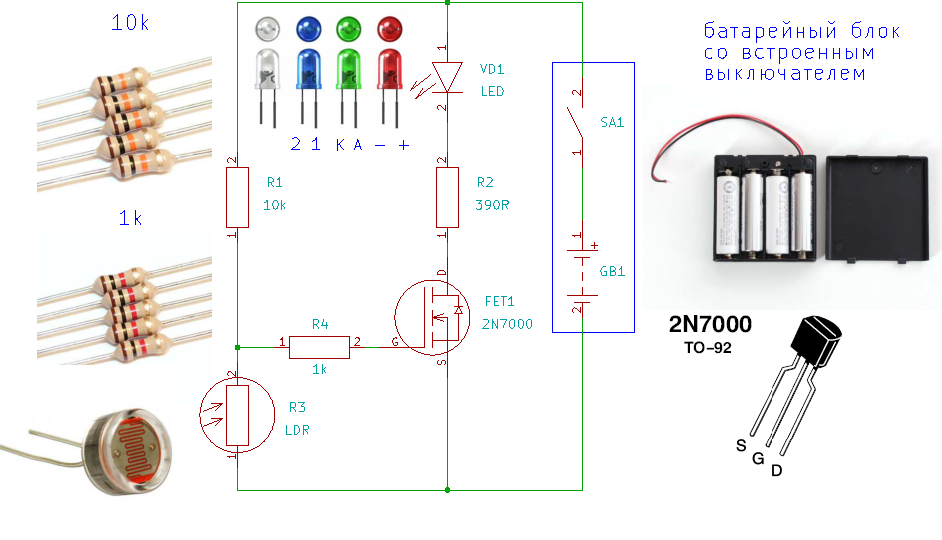
\includegraphics[width=\textwidth]{bcollis/ldr/final.pdf}


\secup
